%%% Local Variables:
%%% mode: latex
%%% TeX-master: t
%%% End:

\documentclass{article}

\usepackage{fullpage}
\usepackage[utf8]{inputenc}
\usepackage{listings}
\usepackage[table]{xcolor}
\usepackage{amssymb}
\usepackage{amsmath}
\usepackage{fancyhdr}
\usepackage{lastpage}
\usepackage{parskip}
\usepackage{abstract}
\usepackage{url}
\usepackage{float}
\usepackage{enumitem}
\usepackage{fancybox}
\usepackage{amsmath}
\usepackage{graphicx}
\usepackage[bottom]{footmisc}
\usepackage{hyperref}
\usepackage{makecell}
\usepackage{tikz}
\usetikzlibrary{arrows,automata}


% constants
\newcommand{\COURSE}{02257 Applied Functional Programming}
\newcommand{\TITLE}{Project 3}
\newcommand{\DATE}{January 20, 2015}


\input{macros}


\pagestyle{fancy}
\fancyhf{}
\setlength{\parindent}{0pt}
\setlength{\headheight}{15pt}
\setlength{\headsep}{25pt}
\lhead{\COURSE}
\chead{\TITLE}
\rhead{\DATE}
\cfoot{Page \thepage{} of~\pageref{LastPage}}


\title{\TITLE\\ {\large \COURSE}}
\date{\DATE}
\author{
  Markus Færevaag {\tt s123692}\\
  Simon Altschuler {\tt s123563}
}


\begin{document}
\maketitle
\vspace{10cm}
\doublesignature{Markus Færevaag}{Simon Altschuler} \\
\clearpage

\section{Introduction}
In this report we will describe our experience with TODO


\section{Status}
TODO

\section{Finite-State Automata}
\begin{figure}[H]
\begin{tikzpicture}[auto, thick, node distance=3.6cm, yscale=2.0]

  \node[initial,state, minimum size=2cm] (ready)                            {{\tt ready}};
  \node[state, minimum size=2cm]         (loading)    [right of=ready]      {{\tt loading}};
  \node[state, minimum size=2cm]         (cancelling) [right of=loading]    {{\tt cancelling}};
  \node[state, minimum size=2cm]         (play)       [right of=cancelling] {{\tt play}};
  \node[state, minimum size=2cm]         (finished)   [right of=play]       {{\tt finished}};

  \path[->] (ready) edge [loop above, yscale=0.5] node {{\tt *}}        (ready)
                    edge                          node {{\tt Load}}     (loading)
          (loading) edge                          node {{\tt Cancel}}   (cancelling)
                    edge [bend left, below]       node {{\tt Loaded}}   (play)
                    edge [bend left, pos=0.2]     node {{\tt Error, *}} (ready)
       (cancelling) edge [bend left, pos=0.2]     node {{\tt *}}        (ready)
             (play) edge [loop above, yscale=0.5] node {{\tt *}}        (play)
                    edge [bend left, pos=0.2]     node {{\tt Cancel}}   (ready)
                    edge                          node {{\tt Finished}} (finished)
         (finished) edge [bend right, above]      node {{\tt Load}}     (loading)
                    edge [bend left, pos=0.2]     node {{\tt *}}        (ready);

\end{tikzpicture}
\caption{Finite-State Automata}
\end{figure}
\end{document}
